\documentclass{beamer}
\usepackage{mathrsfs,xcolor,setspace,comment,centernot,listings,framed,babel,subfig,ragged2e}
\usepackage[utf8]{inputenc}
\usepackage[T1]{fontenc}

\DeclareMathOperator{\Cov}{Cov}
\DeclareMathOperator{\Var}{Var}
\DeclareMathOperator{\E}{\mathbb{E}}
\DeclareMathOperator{\Proba}{\mathbb{P}}

\newcommand{\Covb}[2]{\ensuremath{\Cov\!\left[#1,#2\right]}}
\newcommand{\Eb}[1]{\ensuremath{\E\!\left[#1\right]}}
\newcommand{\Pb}[1]{\ensuremath{\Proba\!\left[#1\right]}}
\newcommand{\Varb}[1]{\ensuremath{\Var\!\left[#1\right]}}

% norm
\newcommand{\norm}[1]{\| #1 \|}

\newcommand{\indep}{\rotatebox[origin=c]{90}{$\models$}}



% config du theme metropolis
\usetheme[progressbar=frametitle,block=fill, titleformat=smallcaps,sectionpage=progressbar,]{metropolis}




\title{Quantifying Co-evolution in Urban Systems with Transfer Entropy}
\subtitle{CCS 2026}
\date{13/10/2026}
\author{Juste Raimbault\textsuperscript{1, 2, 3, 4, $\ast$}}
\institute{\textsuperscript{1}LaSTIG, Université Gustave Eiffel, IGN-Géodata Paris\\
\textsuperscript{2}CASA, UCL\\
\textsuperscript{3}UPS CNRS 3611 ISC-PIF\\
\textsuperscript{4}UMR CNRS 8504 Géographie-cités\\
$\ast$ \texttt{juste.raimbault@geodata-paris.fr}}

\titlegraphic{\vspace{3.5cm}\flushright
\includegraphics[height=2cm,keepaspectratio]{figures/Geodata_Paris.png}} 


%definition de la couleur du texte dans la balise \alert{}
\definecolor{bleuGeodata}{HTML}{2b317f}
\setbeamercolor{alerted text}{fg=bleuGeodata}

%\definecolor{grisIGN}{HTML}{22292F} 
%\setbeamercolor{background canvas}{bg=grisIGN}

\setbeamercolor{frametitle}{fg=bleuGeodata, bg=white}

\makeatletter
\setbeamertemplate{frametitle}{%
  \nointerlineskip%
  \begin{beamercolorbox}[%
      wd=\paperwidth,%
      sep=0pt,%
      leftskip=\metropolis@frametitle@padding,%
      rightskip=\metropolis@frametitle@padding,%
    ]{frametitle}%
  \metropolis@frametitlestrut@start%
  \insertframetitle%
  \nolinebreak%
  \metropolis@frametitlestrut@end%
  \hfill
  \raisebox{-0.6ex}{
\includegraphics[height=4ex,keepaspectratio]{figures/Geodata_Paris.png}}
  \end{beamercolorbox}%
}


\newcommand{\noun}[1]{\textsc{#1}}
\newcommand{\jitem}[1]{\item \begin{justify} #1 \end{justify} \vfill{}}
\newcommand{\sframe}[2]{\frame{\frametitle{#1} #2}}

\newenvironment{centercolumns}{\begin{columns}[c]}{\end{columns}}
%\newenvironment{jitem}{\begin{justify}\begin{itemize}}{\end{itemize}\end{justify}}



\usepackage{pifont}
\newcommand{\cmark}{\ding{51}}
\newcommand{\xmark}{\ding{55}}


\usepackage{multirow}

\makeatother







\begin{document}

%\metroset{background=dark} % change background theme according to manual

\maketitle	






\sframe{Co-evolution between networks and land-use}{

% Understanding urban systems, either from a theoretical viewpoint or for practical sustainable planning applications, often implies intricate dynamics, that can be in some cases with circular causalities between populations of agents or objects, be coined as co-evolution [1]. In particular, the co-evolution between transportation networks and land-use remains quite unknown, despite direct usefulness regarding several Sustainable Development Goals (better accessibility, decarbonised transport, limited urban sprawl).



\begin{center}
  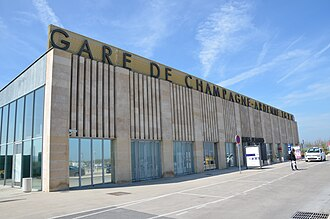
\includegraphics[width=0.33\linewidth]{figures/TGV_Champagne-Ardenne_TGV.jpg}
  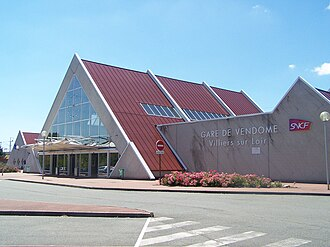
\includegraphics[width=0.3\linewidth]{figures/TGV_Gare_de_Vendome_Villiers-sur-Loir.jpg}
  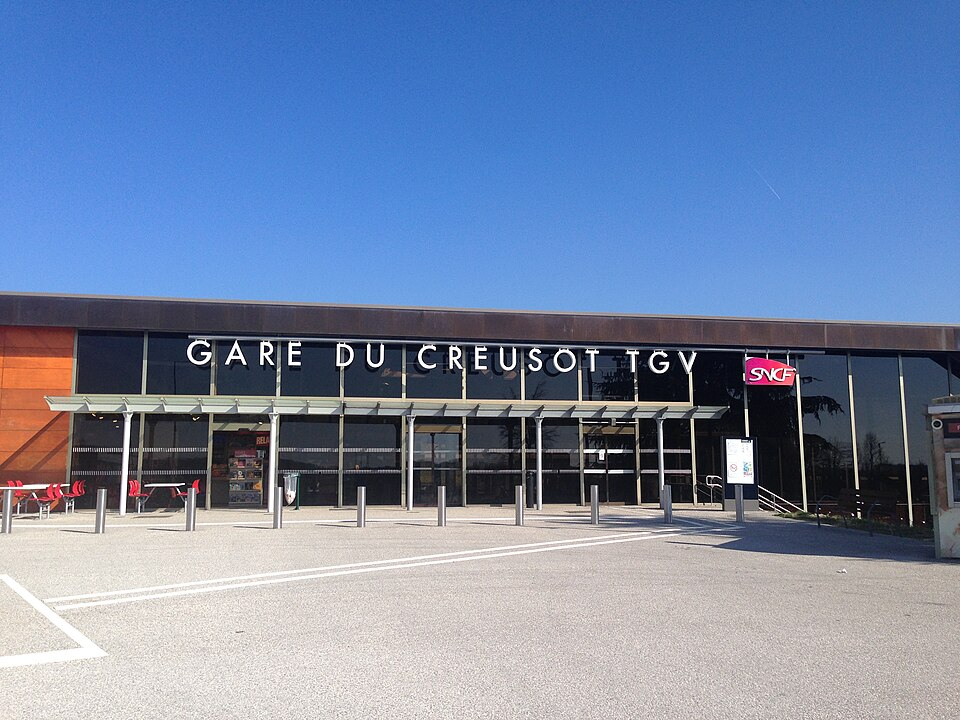
\includegraphics[width=0.3\linewidth]{figures/TGV_LeCreusot.jpg}
\end{center}

\begin{itemize}
	\item Examples of various land-use impacts of new High Speed Rail stations 
\cite{blanquart2017local}
	\item Transportation networks respond to land-use dynamics at other timescales, with governance processes involved \cite{raimbault2021introducing}\cite{le2026modelling} 
\end{itemize}





}


\sframe{Characterising co-evolution in territorial systems}{

% A method to characterise co-evolution, and more generally the structure of the causal graph between the considered urban system variables, and to establish causality regimes either in empirical data or across the parameter space of a simulation model, has been proposed [2], based on Granger causalities.

% - def
% - empirique
% - regimes sur RBD

$\rightarrow$ \cite{raimbault2021characterising} : a definition of co-evolution in territorial systems, transfered from ecology, based on statistical circular causalities on populations of objects


$\rightarrow$ \cite{raimbault2017identification} : a method based on lagged correlations (Granger causality) to identify ``causality regimes''


\begin{columns}
\begin{column}{0.6\linewidth}
\begin{center}
	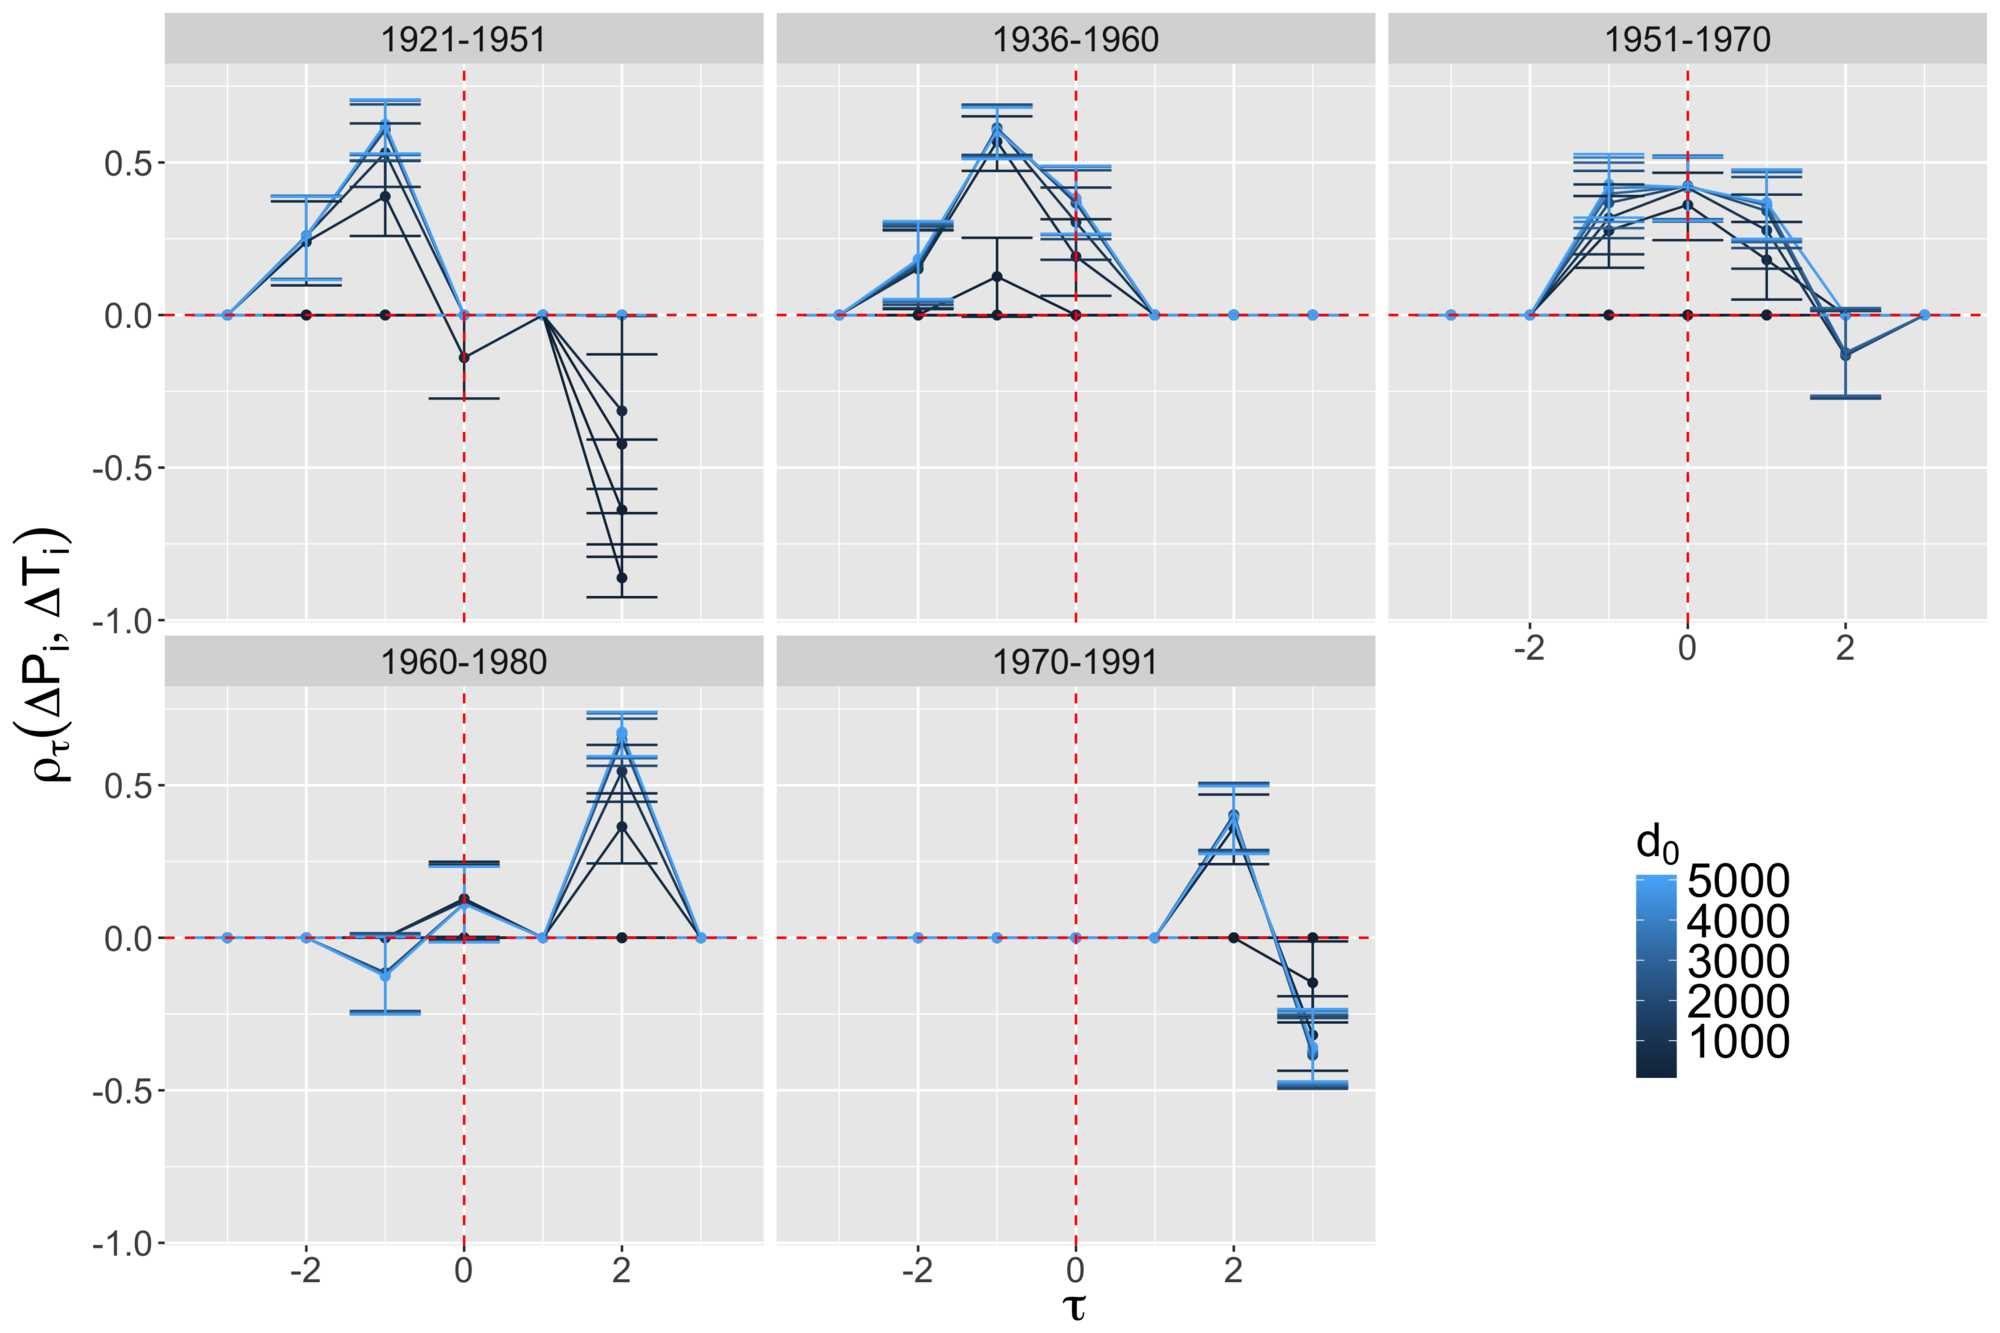
\includegraphics[width=\linewidth]{figures/4-2-3-fig-causalityregimes-sudafcorrs.jpg}
\end{center}
\end{column}
\begin{column}{0.4\linewidth}
$\rightarrow$ various applications to empirical data : railways and urban population, transport projects and real estate prices
\end{column}
\end{columns}


}

\sframe{Causality regimes in co-evolution models}{

% exemple meso et macro

$\rightarrow$ Simulation models with reciprocal interactions between networks and land-use at the micro scale effectively do produce co-evolution in the statistical sense at the macro-scale

\medskip


\begin{columns}
\begin{column}{0.5\linewidth}
\begin{center}
	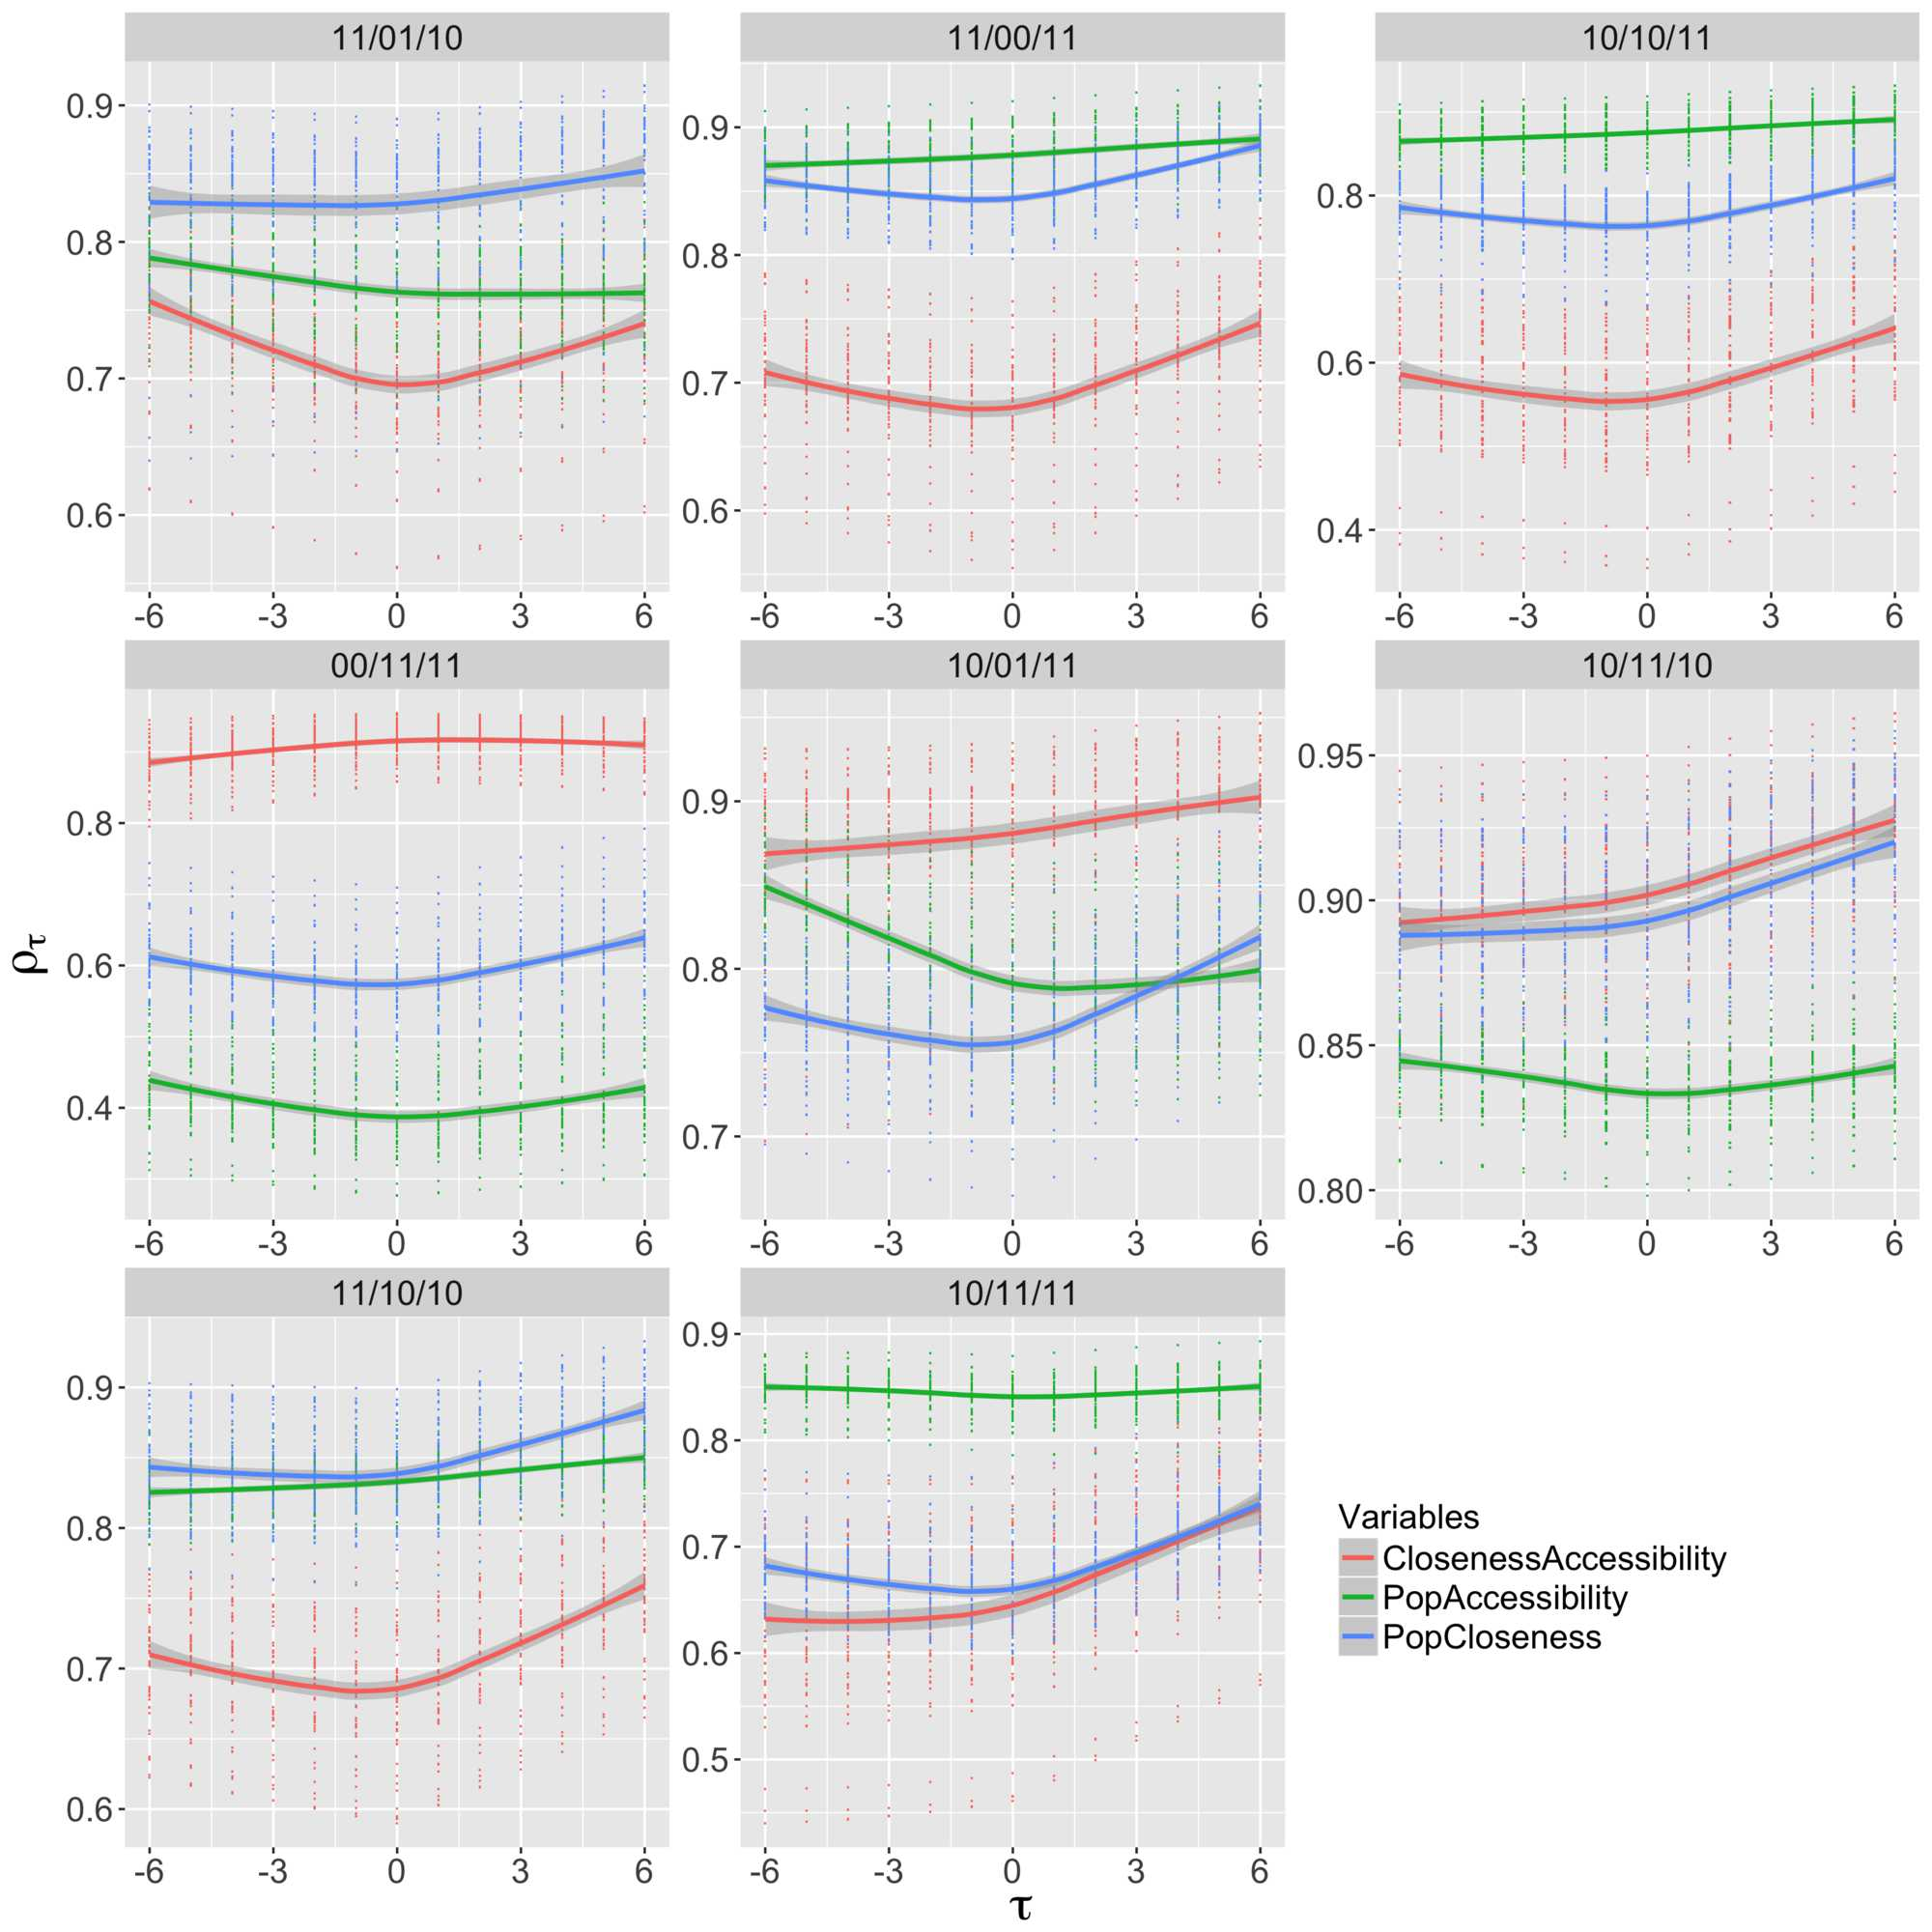
\includegraphics[width=0.85\linewidth]{figures/6-2-2-fig-macrocoevol-correlations.jpg}
\end{center}
\textit{Urban system co-evolution model} \cite{raimbault2021modeling}
\end{column}
\begin{column}{0.5\linewidth}
	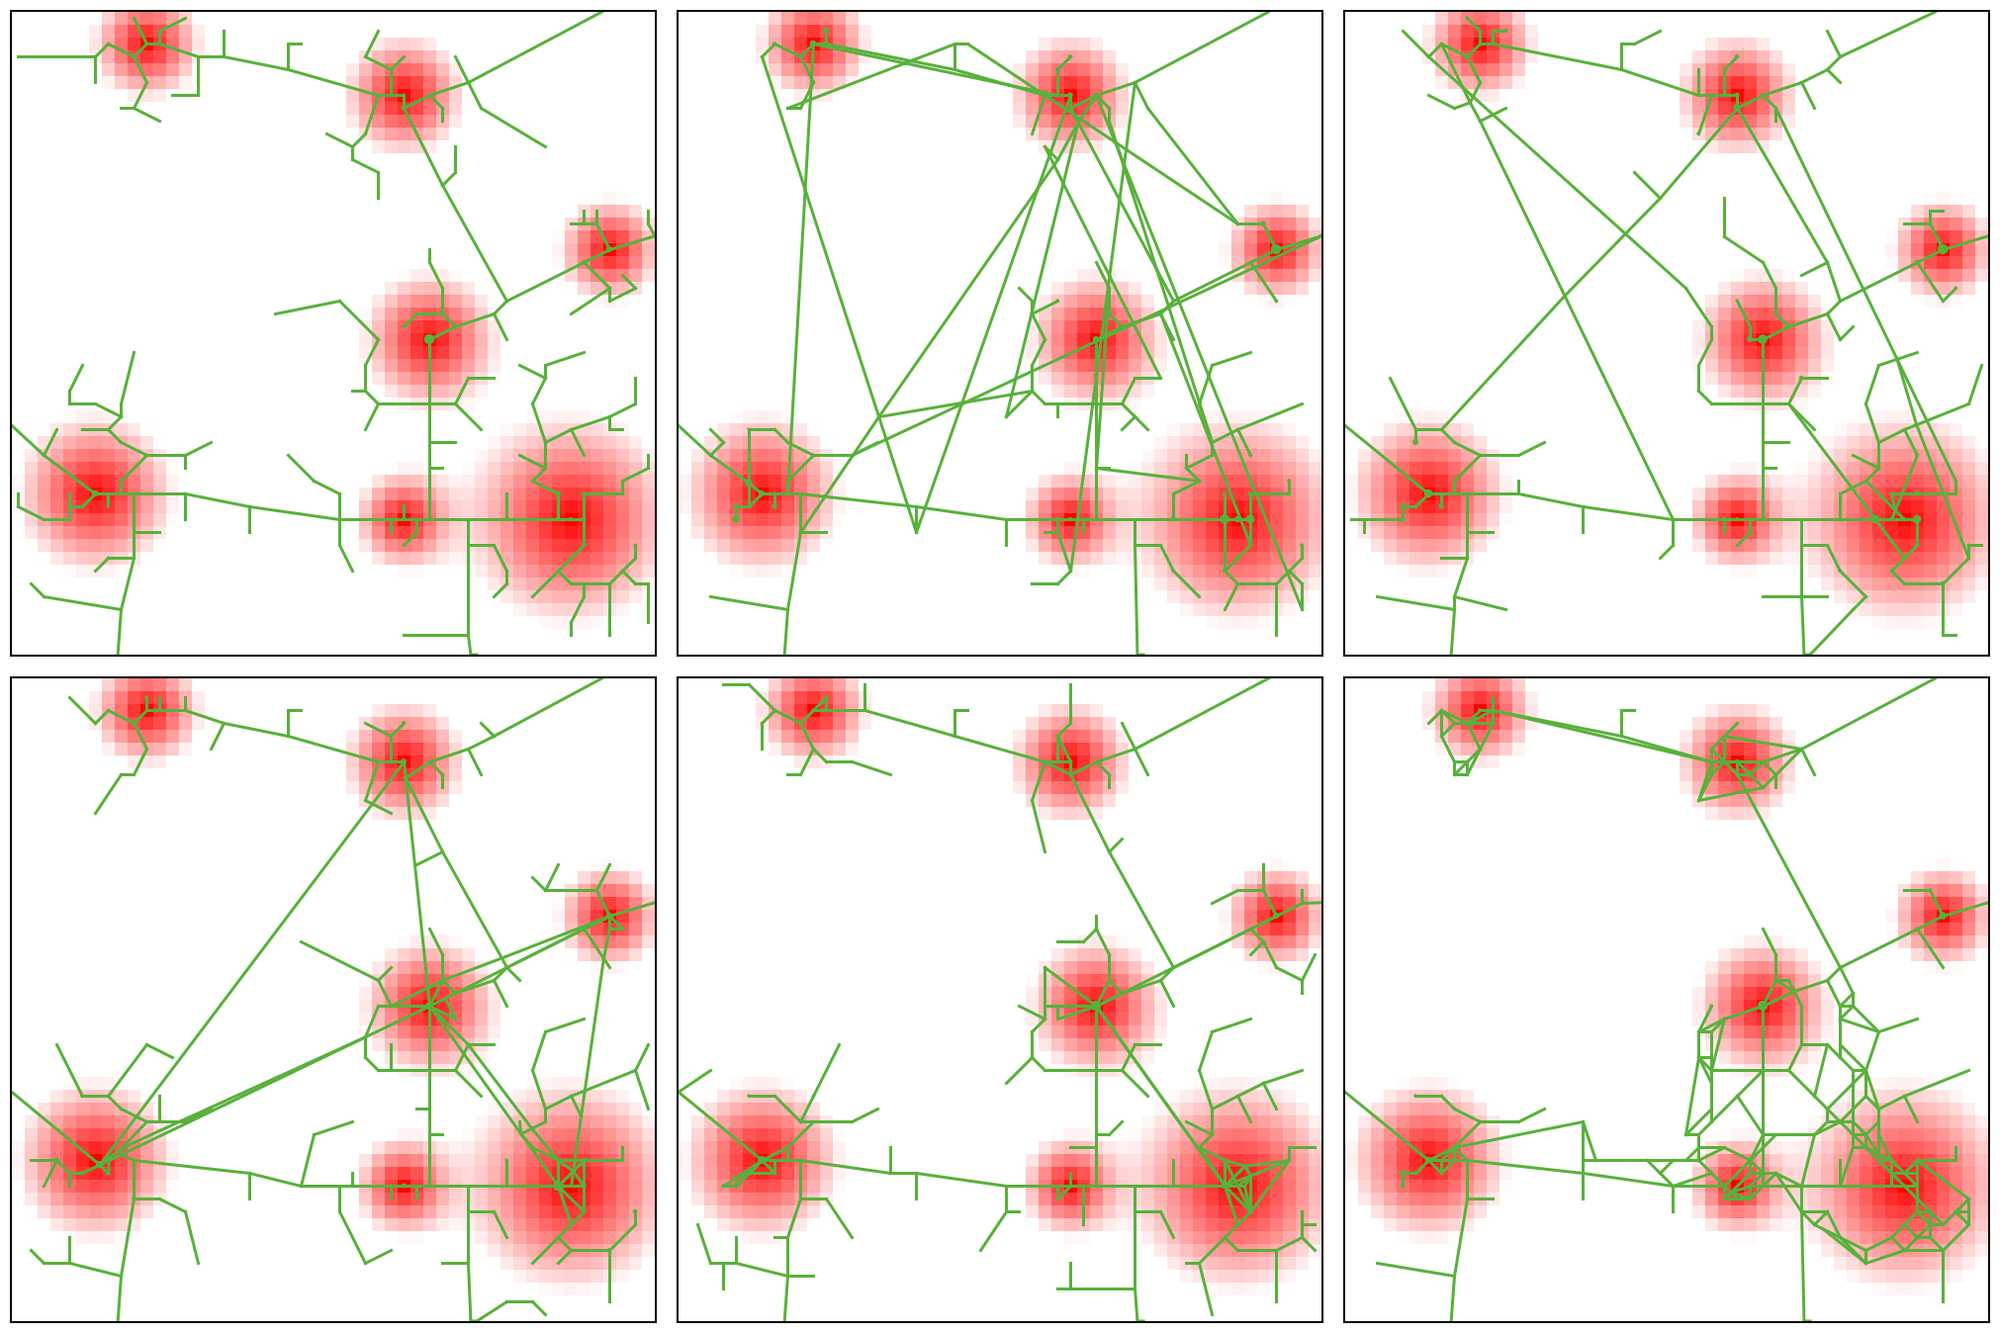
\includegraphics[width=\linewidth]{figures/7-1-2-fig-networkgrowth-examples.jpg}
	
	\textit{Urban morphogenesis co-evolution model} \cite{raimbault2019urban}
\end{column}
\end{columns}


}



\sframe{Extending the method with Information Theory}{

% This contribution investigates how the method can be extended and refined with Transfer Entropy (TE), which provides a more robust and non-linear measure of causality.

% research objective

$\rightarrow$ causality in complex systems estimated with more robust and non-linear approaches, for example based on Information Theory for causality between scales by \cite{rosas2020reconciling}

\medskip

$\rightarrow$ applied to urban systems multi-scale simulation models by \cite{raimbault2023innovation} and \cite{raimbault2026quantifying}

\bigskip

\textbf{Research question : }

\textit{How can measures based on Information Theory, in particular Transfer Entropy, be used to extend the method to identify causality regimes and co-evolution?}


}


\sframe{Method}{

% Given two or more time-series of urban dynamics, observed on a population of objects, Effective Transfer Entropy between all directional couples of variables are estimated on the ensemble (Kraskov estimator implemented in the jidt Java library).

For two variables $X, Y$, Transfer Entropy computed for a delay $\tau$ as

\[
TE_{X \to Y} = I(Y_{t+\tau} ; X_{t}, Y_{t}) - I(Y_{t+\tau} ; Y_{t})
\]

Effective Transfer Entropy is used to remove bias with bootstrapped surrogates :

\[
ETE_{X \to Y} = TE_{X \to Y} - \frac{1}{M}\sum_{m=1}^{M} TE^{(surr,m)}_{X \to Y}
\]

ETE is estimated on an ensemble with a Kraskov estimator (java jidt library implementation \cite{lizier2014jidt}), on the population of urban objects 

}


\sframe{Urban morphogenesis model}{

%We test the method on a stylised yet rich model of urban morphogenesis [3], which simulates settlement and network growth simultaneously, with weight parameters balancing between the explaining factors of future urbanisation (among local density, distance to centre, distance to road network) and with a network growth following a simple connection rule. We compute causalities on the population of raster cells, and density, distance to centre and distance to roads variables.

\footnotesize

\cite{raimbault:halshs-01388885} : a simple and stylised urban morphogenesis model coupling urban development (cellular automaton) with a growing road network, in an iterative way:

\begin{itemize}
	\item $N$ cells with the highest value (weighted average of density, distance to roads, distance to centre) are urbanised
	\item newly urbanised cells too far from the network are connected with a new road on the shortest path
\end{itemize}

\begin{center}
	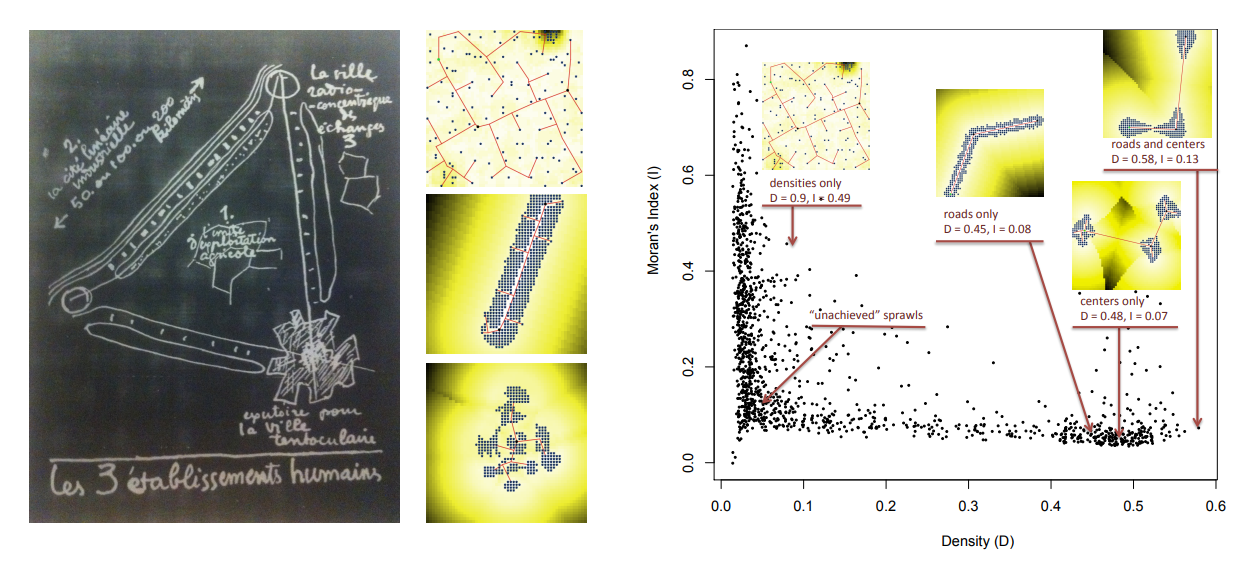
\includegraphics[width=\linewidth]{figures/RaimbaultBanosDoursat2014_Fig3-4.png}
\end{center}

}


\sframe{Implementation and experiments}{


\footnotesize

$\rightarrow$ models implemented in \texttt{NetLogo}, with the Transfer Entropy calculation from the \texttt{jidt} Java library integrated as an extension

\smallskip

$\rightarrow$ integration into the OpenMOLE model exploration and validation open source software \cite{reuillon2013openmole} (\textit{seamless (i) model embedding; (ii) access to HPC resources; (iii) exploration and optimisation algorithms})


\begin{center}
\includegraphics[height=0.13\textheight]{../../../../../../UrbanSystems/UrbanGrowth/Docs/Communications/2019/CCS2019/Communication/figures/iconOM.png}
\includegraphics[height=0.13\textheight]{../../../../../../UrbanSystems/UrbanGrowth/Docs/Communications/2019/CCS2019/Communication/figures/openmole.png}
\end{center}


\smallskip

$\rightarrow$ urban morphogenesis model run on synthetic systems of cities \cite{raimbault2019space}, with default model parameters

\smallskip

$\rightarrow$ a grid parameter sampling (step 0.5) is done on weights parameters ($w_{density}$, $w_{roads}, w_{centre}$) with 10 repetitions ; ETE computed on all couples of cell value variables (density, distance to roads, distance to centre), with $1 \leq \tau \leq 3$


}



\sframe{Examples of causality regimes}{

% A first experiment, a grid exploration of the model parameter space, provide a broad set of causality regimes, with some illustrated in Fig. 1. 

\begin{center}
	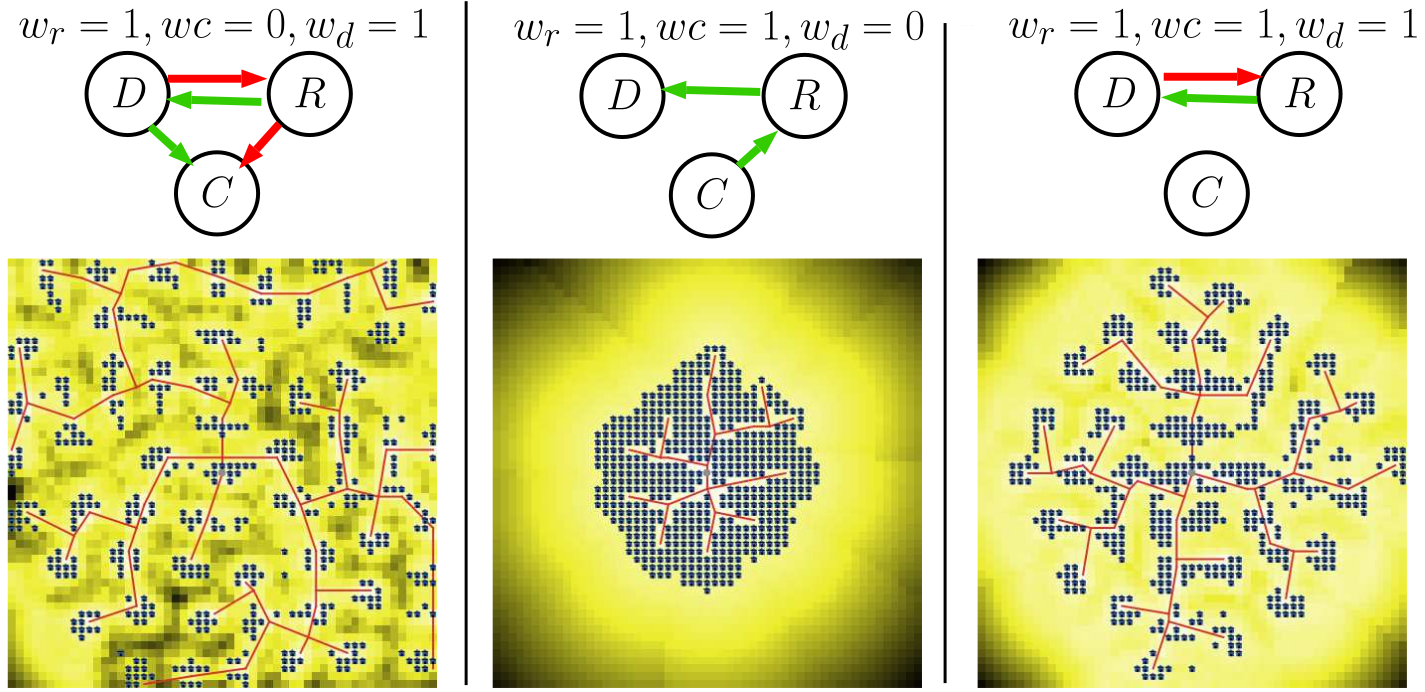
\includegraphics[width=\linewidth]{figures/Fig1.png}
\end{center}

\textit{Examples of Granger causality regimes previously obtained in \cite{raimbault2021characterising}}

}

\sframe{Results with Transfer Entropy}{

% The TE method appears more systematic and robust than the previous method, with some regimes not found significant by lagged correlations before.

\begin{columns}
	\begin{column}{0.7\linewidth}
		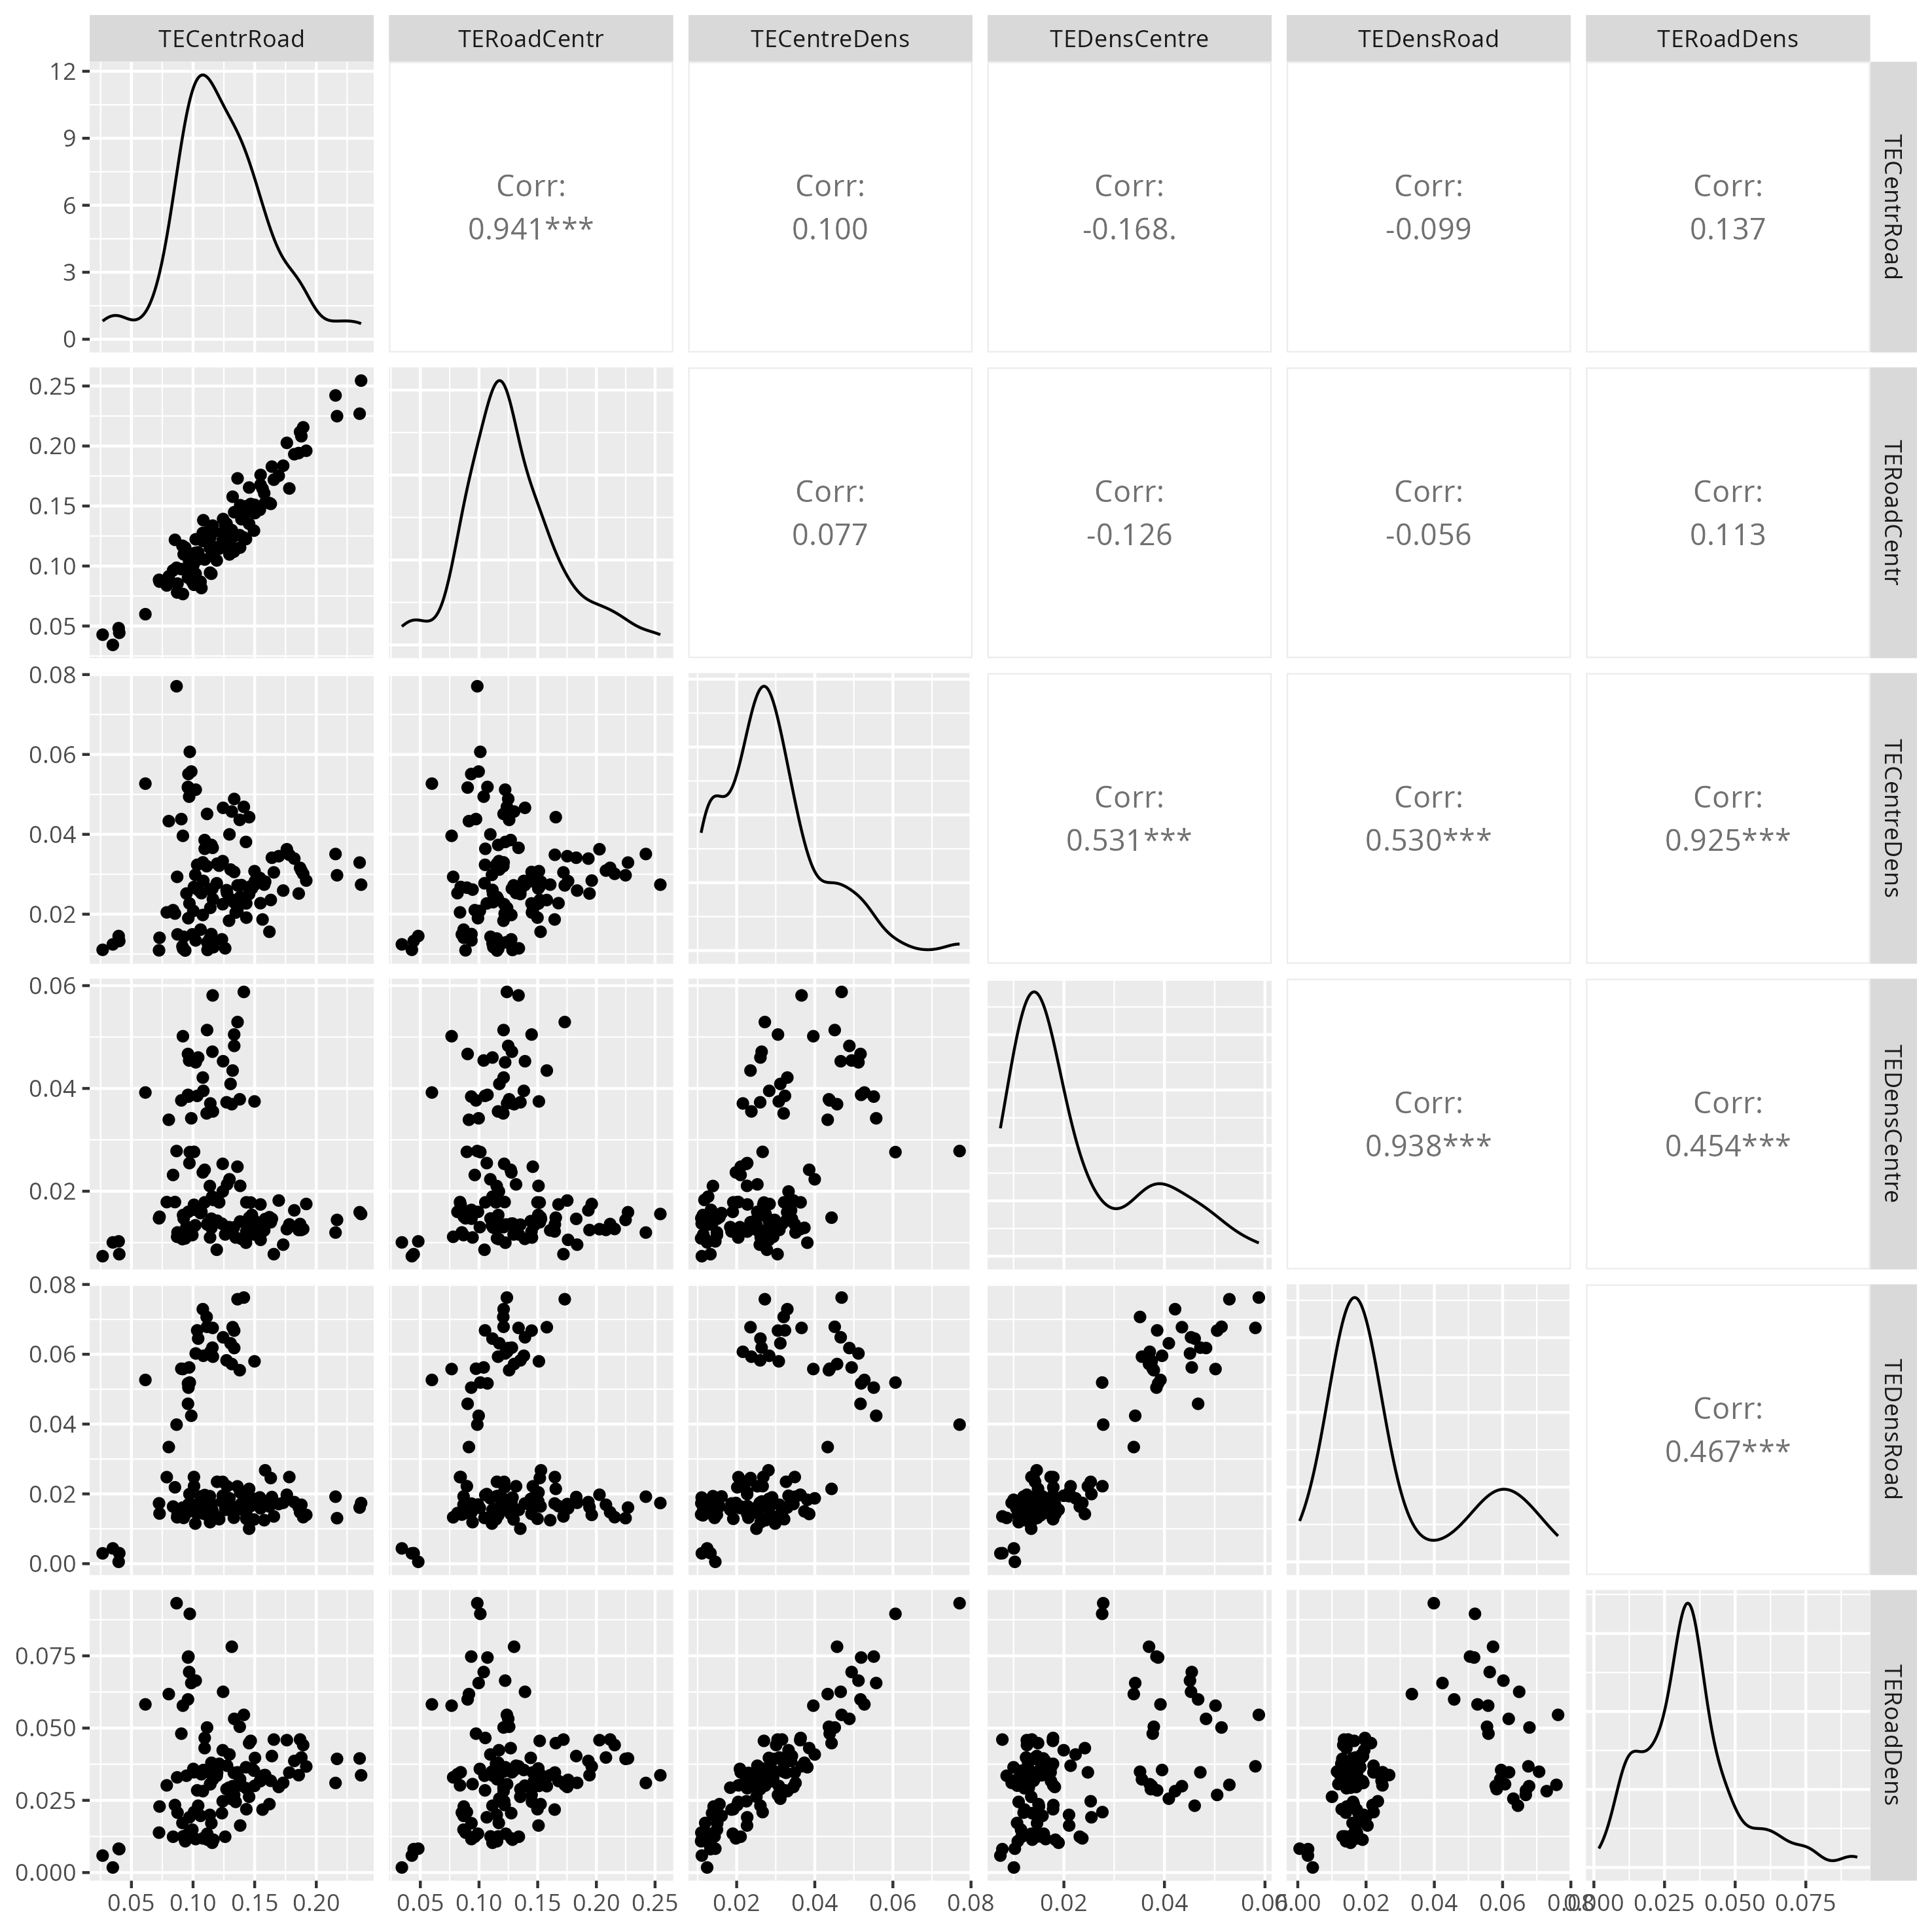
\includegraphics[width=\linewidth]{figures/TE-scatterplot.png}
	\end{column}
	\begin{column}{0.3\linewidth}
% TE regimes on 119 simulated cities
%         0         1         2         3 
%  35.294118 32.773109 27.731092  4.201681 

	\footnotesize
	\justify	

	Proportion of regimes, by number of reciprocal causalities (ETE in both directions larger than its median)
	\begin{enumerate}
		\item[0] : 35\%
		\item[1] : 33\%
		\item[2] : 28\%
		\item[3] : 4\%
	\end{enumerate}


	% correlations
	%         0         1         2         3 
	%	42.152466 34.080717 22.421525  1.345291 

	\bigskip

	With lagged correlations
	
	\begin{enumerate}
		\item[0] : 42\%
		\item[1] : 34\%
		\item[2] : 22\%
		\item[3] : 1\%
	\end{enumerate}
	
	\end{column}
\end{columns}

}




\sframe{Discussion}{

%      This confirms that TE is an appropriate tool to quantify co-evolution in urban systems, to be further tested on more cases.


% - work in progress : PSE 
% run the PSE algorithm \cite{cherel2015beyond} on emergence indicators

\justify
\footnotesize

$\rightarrow$ a proof-of-concept of extending the causality regimes/coevolution method with Transfer Entropy

\medskip

\textbf{Work in progress}

\begin{itemize}
	\item Statistical validation, larger sampling, interpretation of regimes
	\item Pattern Search Exploration algorithm to explore the feasible space of causality regimes \cite{cherel2015beyond}
\end{itemize}

\medskip

\textbf{Future work}

\begin{itemize}
	\item Test on empirical data %same difficulties than with lagged correlations: lack of data, identification problems -> ignore it in some sense, as not stat model but purely empirical "correlations"?
	\item Systematic benchmark of co-evolution models \cite{le2026modelling}
\end{itemize}

\bigskip

Code and data available at

\url{https://github.com/JusteRaimbault/CoevolutionNwTerritories/tree/master/Models/MesoCoevolCA}


}





%%%%%%%%%%%%%%%%%%%%%
\begin{frame}[allowframebreaks]
\frametitle{References}
\bibliographystyle{apalike}
\bibliography{biblio.bib}
\end{frame}
%%%%%%%%%%%%%%%%%%%%%%%%%%%%



\end{document}




